\begin{gather*}
\sum_{n\leq x}\frac1n = \log x + \gamma + O(\tfrac1x) \\
\sum_{n\leq x}\frac1{n^a} = \zeta(a) - \frac{1}{(a-1)x^{a-1})} + O(\tfrac1x) \\
\sum_{n\leq x}\log n = x\log x - x + O(\log x)
\end{gather*}
\eg Find an asymptotic formula for $\sum_{n\leq x}\tau(n)$ \\
\soln
\[ \sum_{n\leq x} \tau(n) = \sum_{n\leq x}\sum_{d\div n}1 \]
%[diagram]
\begin{center}
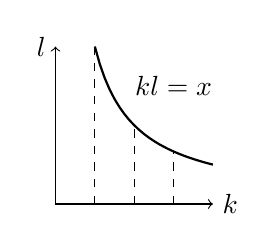
\begin{tikzpicture}[domain=0.5:2]
%\draw[gray,very thin](0,0) grid (2,2);
\draw[thick] plot(\x,1/\x);
\draw[dashed] (0.5,0)--(0.5,2);
\draw[dashed] (1,0)--(1,1);
\draw[dashed] (1.5,0)--(1.5,1/1.5);
\draw[<->] (0,2) node[left]{$l$}--(0,0)--(2,0) node[right]{$k$};
\node at (1.5,1.5) {$kl=x$};
\end{tikzpicture}
\end{center}
\begin{align*}
\sum_{\substack{k,l\\kl\leq x}}1 &= \sum_{k\leq x}\sum_{l\leq\frac{x}{k}}1 \\
&= \sum_{k\leq x}\floor*{\frac{x}{k}} = \sum_{k\leq x}\paren*{\frac{x}{k}-\chev*{\frac{x}{k}}} \\
&= x \sum_{k\leq x}\frac1k - \sum_{k\leq x}\chev*{\frac{x}{k}} \\
&= x(\log x+\gamma+O(\tfrac1x)) + O(x)\footnote{since
\[ \sum_{k\leq x}\chev*{\frac{x}{k}} \leq \sum_{k\leq x}1 = \floor{x} = x - \chev{x} = x + O(1) \]} \\
&= x\log x + \gamma x + O(1) + O(x) \\
&= x\log x + O(x)
\end{align*}
\eg Find a better one
\begin{align*}
\soln \sum_{n\leq x}\tau(n) &= \sum_{n\leq x}\sum_{d\div n}1 \\
&= \sum_{\substack{k,l\\kl\leq x}}1 \\
&= \sum_{k^2\leq x}1 + 2\sum_{k\leq\sqrt x}\sum_{k<l\leq\frac xk}1 \\
&= \sum_{k\leq\sqrt x}1 + 2\sum_{k\leq\sqrt x}\paren[\Big]{\sum_{l\leq\frac xk}1-\sum_{l\leq k}1} \\
&= \floor{\sqrt{x}} + 2 \sum_{k\leq\sqrt x}\paren[\Big]{\floor[\Big]{\frac xk}-k} \\
&= (\sqrt{x}+O(1)) + 2\sum_{k\leq\sqrt x}\paren[\Big]{\frac xk + O(1) - k} \\
&= \sqrt{x} + O(1) + 2x\sum_{k\leq\sqrt x}\frac1k-2\sum_{k\leq\sqrt x}k+2O(1)\sum_{k\leq\sqrt x}1 \\
\sqrt{x} + O(1) + 2x(\log\sqrt x+\gamma+O(\tfrac1x)) \\ {}- 2\frac{\floor{\sqrt x}(\floor{\sqrt x}+1)}{2} + O(\sqrt x) %\\
&= \sqrt x + x\log x + 2\gamma x + O(\sqrt x) - (\sqrt x+O(1))(\sqrt x+O(1)) \\
&= x\log x + 2\gamma x - x + O(\sqrt x) \\
&= x\log x + (2\gamma-1)x + O(\sqrt x)
\end{align*}
\eg Find an asymptotic formula for $\sum_{n\leq x}\sigma(n)$.
\begin{align*}
\soln \sum_{n\leq x}\sigma(n) &= \sum_{n\leq x}\sum_{d\div n}d \\
&= \sum_{\substack{k,l\\kl\leq x}}l = \sum_{k\leq x}\sum_{l\leq\frac xk}l \\
&= \sum_{k\leq x}\frac{\floor{\frac xk}(\floor{\frac xk}+1)}{2} \\
&= \frac12\sum_{k\leq x}\paren[\Big]{\frac xk+O(1)}\paren[\Big]{\frac xk+O(1)} \\
&= \frac12\sum_{k\leq x}\paren[\Big]{\frac{x^2}{k^2}+\frac{2x}{k}O(1)+O(1)} \\
&= \frac{x^2}{2}\sum_{k\leq x}\frac1{k^2} + xO(1)\sum_{k\leq x}\frac1k + O(1)\sum_{k\leq x}1 \\
&= \frac{x^2}{2}\paren[\Big]{\zeta(2)-\frac1x+O(\frac1{x^2})} + O(x)(\log x+O(1)) + O(x) \\
&= \frac{x^2}{2}\zeta(2) - \frac{x}{2} + O(1) + O(x\log x) \\
&= \frac{x^2}{2}\zeta(2) + O(x\log x) = \frac{\pi^2}{12}x^2 + O(x\log x)
\end{align*}
\ex Find $\sum_{n\leq x}\sigma_a(n)=\sum_{n\leq x}\sum_{d\div n}d^a$ for $a>1$ \\
\eg Find an asymptotic formula for $\sum_{n\leq x}\phi(n)$.
\begin{align*}
\soln \sum_{n\leq x}\phi(n) &= \sum_{n\leq x}\sum_{d\div n}\frac{\mu(d)n}{d}\footnotemark \\
&= \sum_{\substack{k,l\\kl\leq x}}\frac{\mu(k)kl}{k} = \sum_{\substack{k,l\\kl\leq x}}\mu(k)l \\
&= \sum_{k\leq x}\paren[\Big]{\mu(k)\sum_{l\leq\frac xk}l} \\
&= \sum_{k\leq x}\mu(k)\frac{\floor{\frac xk}(\floor{\frac xk}+1)}{2} \\
&= \frac12\sum_{k\leq x}\mu(k)\paren[\Big]{\frac xk+O(1)}\paren[\Big]{\frac xk+O(1)} \\
&= \frac12\sum_{k\leq x}\mu(k)\paren[\Big]{\frac{x^2}{k^2}+\frac{x}{k}O(1)+O(1)} \\
&= \frac{x^2}{2}\sum_{k\leq x}\frac{\mu(k)}{k^2} + O(x)\sum\frac{\mu(k)}{k} + O(1)\sum_{k\leq x}\mu(k) \\
&= \frac{x^2}{2}\paren[\Big]{\sum_{k=1}^\infty\frac{\mu(k)}{k^2}-\sum_{k>x}\frac{\mu(k)}{k^2}} + O(x\log x)\footnotemark + O(x) \\
&= \frac{x^2}{2}\paren[\Big]{\frac{1}{\zeta(2)}+O(\tfrac1x)}\footnotemark + O(x\log x) \\
&= \frac{x^2}{2}\cdot\frac{1}{\zeta(2)} + O(x) + O(x\log x) \\
&= \frac{3}{\pi^2}x^2 + O(x\log x)
\end{align*}\addtocounter{footnote}{-2}\footnotetext{Recall:
\begin{gather*}
N(n) = n = \sum_{d\div n}\phi(d) \\
\phi(n) = \sum_{d\div n}\frac{\mu(d)n}{d}
\end{gather*}}\addtocounter{footnote}{1}\footnotetext{since
\[ \abs[\Big]{\sum_{k\leq x}\frac{\mu(k)}{k}} \leq \sum_{k\leq x}\frac1k = \log x + O(1) = O(\log x) \]
and
\[ \abs[\Big]{\sum_{k\leq x}\mu(k)} \leq \sum_{k\leq x}1 = \floor{x} = x - \chev{x} = x + O(1) = O(x) \]}\addtocounter{footnote}{1}\footnotetext{since
\[ \abs[\Big]{\sum_{k>x}\frac{\mu(k)}{k^2}} \leq \sum_{k>x}\frac1{k^2} \leq \int_{x-1}^\infty \frac1{t^2}\d t = \frac{1}{x-1} = O\paren[\Big]{\frac1x} \]}%
Next: $\sum\frac{\Lambda(n)}{n}=\log x+O(?)$ \\
$\sum_{p\leq x}\frac{\log p}{p}=\log x+O(?)$ \\
$\sum_{p\leq n}\frac1p=\log\log x+O(?)$
